\section{Mod\`ele \`a un seul pool de matière organique}
\subsection{Description du mod\`ele}

\par{
Comme toujours on commence par la description du modèle le plus simple. Dans ce cas, c'est le modèle
\`a un seul pool de matière organique. Cette matière ($TOC$ \~ Carbon Organique Total biodégradable)
est transformée par l'hydrolyse en $SBC$ (Substrats Carbonés monomériques). Ensuite le $SBC$ est
utilisé par les $BC$ (~ bactéries) pour leur croissance. Les bactéries existantes influencent le $NH_4$
(~ ammonium) présent. Le modèle complet est représenté par le schéma conceptuel montre dans la
figure~\ref{fig:partie1concModel}. Ainsi, les équations appartiennent au modèle sont les suivantes:
}

\begin{figure}[h!]
  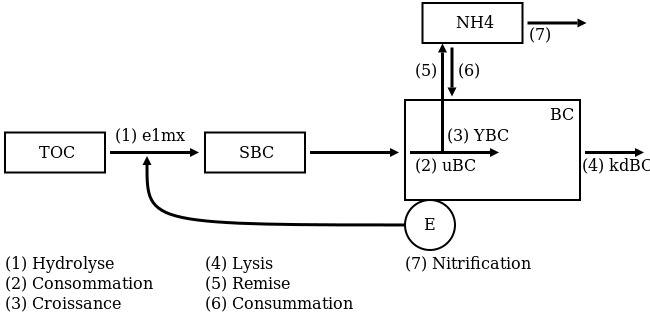
\includegraphics[width=\textwidth]{partie1/scan1.jpg}
  \caption{Le modèle conceptuel du système étudié dans le cinquième cours. Dans le système le pool du
$TOC$ est ectohydrolyse en $SBC$ \textcircled{1}. Cette réaction dépend de la température. Ensuite, 
les bactéries uptake le $SBC$ \textcircled{2}. Cette réaction dépend de la température également. Les
bactéries ont besoin du $SBC$ pour leur croissance. Naturellement le carbone consomme ne peut pas être
utilisée completement pour la croissance. Une certain partie est besoin pour les procédés de
respiration. La partie du carbone inutilisable pour la croissance est représenté par $Y_{BC}$ \textcircled{3}.
Afin de réduire l'augmentation de la concentration des bactéries, le modèle contient une terme pour la lyse
cellulaire des bactéries \textcircled{4}. Les bactéries affectent la concentration en $NH_4$ -
elles absorbent du $NH_4$ pour leurs processus métaboliques \textcircled{6}, mais elles peuvent aussi le
produire \textcircled{5}. Une partie de $NH_4$ est retiré du modèle par nitrification \textcircled{7}.
}
  \label{fig:partie1concModel}
\end{figure}

\begin{equation}
  {{d[BC]}\over{dt}} =
  \left ( Y_{BC} u_{BC} - kd_{BC} \right ) [BC]
  \label{eq:eq1}
\end{equation}
\begin{equation}
  {{d[TOC]}\over{dt}} =
  -ec [BC]
  \label{eq:eq2}
\end{equation}
\begin{equation}
  {{d[SBC]}\over{dt}} =
  ec [BC] - u_{BC} [BC]
  \label{eq:eq3}
\end{equation}
\begin{equation}
  {{d[SNH_4]}\over{dt}} =
  vNH_4 - nitri
  \label{eq:eq4}
\end{equation}

\par{
Avec
}

\begin{equation}
  ec = e_{1mx} {{[TOC]}\over{k_{1h} + [TOC]}}
  \label{eq:eq5}
\end{equation}
\begin{equation}
  vNH_4 = u_{BC} [BC] (NC)_{TOC} - Y_{BC} u_{BC} [BC] (NC)_{BC}
  \label{eq:eq6}
\end{equation}
\begin{equation}
  nitri = nimax {{[NH_4]}\over{k_{NH_4ni}+[NH_4]}}
  \label{eq:eq7}
\end{equation}

\par{
Pour mieux comprendre les équations du modèle, la grille~\ref{tab:partie1descVars} peut également être
intéressante. Elle donne un aperçu de la signification etc. de chaque terme dans les équations.
}

\begin{table}[h!]
\begin{center}
\begin{tabular}{ | c | c | c | c | c | }
\hline
Terme & Signification & Type & Valeur & Unité \\
\hline
$BC$ & \pbox{4cm}{La concentration des bactéries} & Variable d'état & $1$ & ${{mmol~C}\over{m^{-3}}}$ \\
$TOC$ & \pbox{4cm}{La concentration du carbon organique total biodégradable} & Variable d'état & $50$ & ${{mmol~C}\over{m^{-3}}}$ \\
$SBC$ & \pbox{4cm}{La concentration du substrats carbonés monomériques} & Variable d'état & $2$ & ${{mmol~C}\over{m^{-3}}}$ \\
$NH_4$ & \pbox{4cm}{La concentration du l'ammonium} & Variable d'état & $6$ & ${{mmol~N}\over{m^{-3}}}$ \\
$e_{1mx}$ & \pbox{4cm}{Ectohydrolyse à température optimale} & Paramètre & $16$ & $Jours^{-1}$ \\
$k_{1h}$ & \pbox{4cm}{Constante de hydrolyse} & Paramètre & $20$ & ${mmol~C}\over{m^{-3}}$ \\
$b_{maxo}$ & \pbox{4cm}{Uptake $SBC$ à température optimale} & Paramètre & $14$ & $Jours^{-1}$ \\
$ks_{BC}$ & \pbox{4cm}{Constante d'uptake $SBC$} & Paramètre & $2$ & ${{mmol~N}\over{m^{-3}}}$ \\
$T_{opt}$ & \pbox{4cm}{La température optimale des bactéries} & Paramètre & $30$ & $^{\circ}C$ \\
$d_{opt}$ & \pbox{4cm}{delta T} & Paramètre & $18$ & $^{\circ}C$ \\
$Y_{BC}$ & \pbox{4cm}{Taux de croissance} & Paramètre & $0.2$ & - \\
$kd_{BCo}$ & \pbox{4cm}{Taux de mortalité à température optimale} & Paramètre & $0.25$ & $Jour^{-1}$ \\
$ni_{mx}$ & \pbox{4cm}{Vitesse maximale de la nitrification} & Paramètre & $5$ & ${{mmol~N}\over{m^{-3}}}$ \\
$N/C_{(TOC)}$ & \pbox{4cm}{Rapport N:C de $TOC$} & Constant & $^{16} / _{106}$ & ${mmol~N}\over{mmol~C}$ \\
$N/C_{(BC)}$ & \pbox{4cm}{Rapport N:C des $BC$} & Constant & $^{1} / _{4.6}$ & ${mmol~N}\over{mmol~C}$ \\
\hline
\end{tabular}
\end{center}
  \caption{Signification, type, valeur et unité de chaque terme/paramètre des équations du modèle.}
  \label{tab:partie1descVars}
\end{table}

\FloatBarrier
\subsection{Simulation de r\'ef\'erence}

\begin{figure}[h!]
  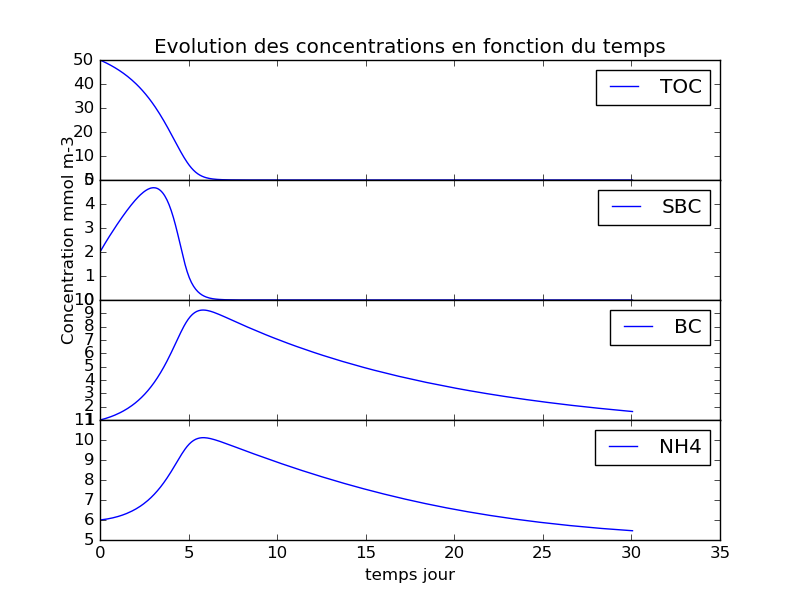
\includegraphics[width=\textwidth]{partie1/Ref.png}
  \caption{Simulation de r\'ef\'erence, pour un mod\`ele \`a un seul pool de mati\`ere organique.
  }
  \label{fig:partie1ref}
\end{figure}

\par{
La figure~\ref{fig:partie1ref} décrit la simulation de référence. 
Sur le graphique de l'\'evolution de la concentration du TOC en fonction du temps, nous pouvons observer que
la concentration d\'ecro\^it de 0 \`a 6 jours et atteint une valeur nulle apr\`es 6 jours. En effet, ce TOC
est hydrolys\'e en SBC, qui d\'epend de la concentration en bact\'eries et de la concentration en TOC. Ainsi,
au d\'ebut de la simulation, la d\'ecroissance du TOC est due \`a la grande concentration en TOC (car la
valeur de ec est grande). Ensuite, la d\'ecroissance de la concentration de TOC est due \`a une augmentation
de la concentration en bact\'eries.
}
\par{
Sur le graphique de l'\'evolution de la concentration en SBC, on peut voir que sa concentration augmente de
0 \`a 4 jours, ou elle atteint une valeur maximale de 4,8 mmolC.m-3, puis d\'ecroit de 4 \`a 6 jours,
jusqu'\`a atteindre une valeur nulle. En effet, l'\'evolution de la concentration en SBC est due \`a la
concentration en TOC et en SBC. Ainsi, au d\'ebut de la simulation, la concentration en TOC est importante,
et celle en SBC est faible, et donc, le terme d'augmentation de la concentration est sup\'erieur au terme de
diminution. A 4 jours, les deux termes s'\'egalisent, car la concentration en TOC diminue et car la
concentration en SBC augmente. Finalement, apr\`es 4 jours, le terme de diminution de la concentration en SBC
diminue jusqu'\`a atteindre une valeur nulle, un peu apr\`es que le TOC atteigne une valeur nulle.
}
\par{
Sur le graphe de l'\'evolution de la concentration en bact\'eries, on peut observer que celle-ci augmente de
0 \`a 6 jours, atteint une valeur maximale de de 9 mmolC.m-3, puis d\'ecro\^it. En effet, l'\'evolution de
cette concentration d\'epend de la concentration en SBC. Ainsi, au d\'ebut de la simulation la concentration
en SBC augmente, et donc la concentration en bact\'eries augmentent aussi, car le terme de croissance
l'emporte sur le terme de mortalit\'e. Au maximum de concentration, les deux termes se compensent, car la
concentration en SBC diminue. Finalement, la concentration en SBC devient nulle, et donc seul le terme de
mortalit\'e influence l'\'evolution de la concentration en bact\'eries.
}
\par{
Sur le graphe de l'\'evolution de la concentration en NH4, celle-ci augmente de 0 \`a 6 jours, pour atteindre
un maximum de 10 mmolC.m-3, puis d\'ecro\^itre ensuite. En effet, l'\'evolution de la concentration d\'epend
de deux termes: une terme d\'ependant de ce qu'utilise les bact\'eries, par rapport \`a ce dont elles ont
besoins (vNH4, d\'ependant de la concentration en bact\'eries et de la concentration en SBC), et un terme
de nitrification, d\'ependant de la concentration en NH4. Au d\'ebut de la simulation, la concentration en
NH4 augmente, ce qui veut dire que la valeur de vNH4 est sup\'erieur au terme de nitrification. Ainsi, le terme
vNH4 est toujours positif, ce qui signifie que ce qu'utilisent les bact\'eries est toujours sup\'erieur \`a ce
qu'elles ont besoin, et donc qu'elles rejettent du NH4 dans leur environnement. Au maximum de concentration
en NH4, les deux termes se compensent, car la concentration en SBC diminue. Finalement, lorsque la
concentration en SBC devient nulle, l'\'evolution de NH4 ne d\'epend plus que de la nitrification.
}

\FloatBarrier
\newpage
\subsection{Tests de sensitivit\'e}
\subsubsection{Test 1}

\begin{figure}[h!]
  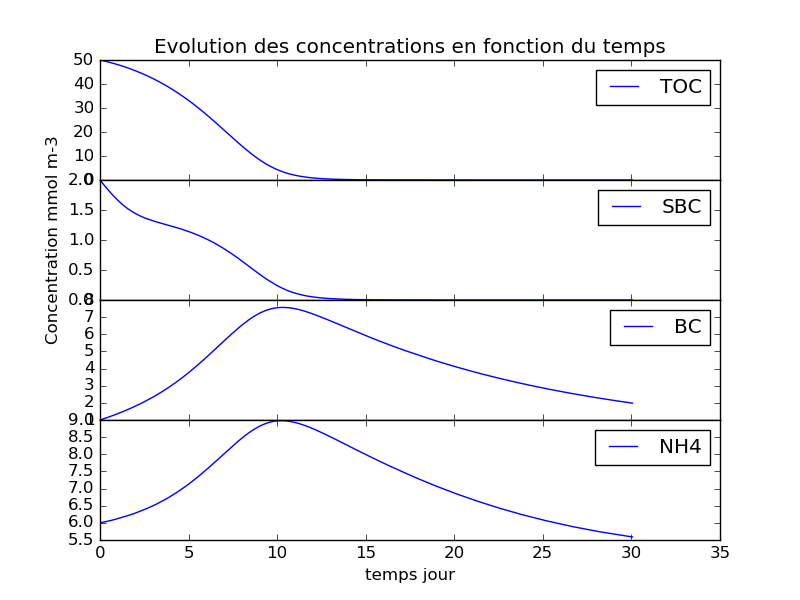
\includegraphics[width=\textwidth]{partie1/Test1.png}
  \caption{Simulation en divisant par deux la valeur de la constante d'ectohydrolyse de TOC \`a temp\'erature optimale.
  }
  \label{fig:partie1test1}
\end{figure}
\par{
Dans le première test en a diminué la constant d'ectohydrolyse à la température optimale en comparison avec
la simulation de référence. Du coup le TOC est moins consumer par le BC. En consequence la valeur du terme
ec diminuera moins vite. Donc, les concentrations maximas des bactéries et des ammonium est atteindent
plus tard. (Le maximum des bactéries est obtenu à $t=10.32$ avec une concentration de
$7.568 {^{mmol~C}/_{m^{-3}}}$ et le maximum d'ammonium est à $10.2$ avec une concentration de
$8.98 {^{mmol~N}/_{m^{-3}}}$.)
}

\FloatBarrier
\newpage
\subsubsection{Test 2}

\begin{figure}[h!]
  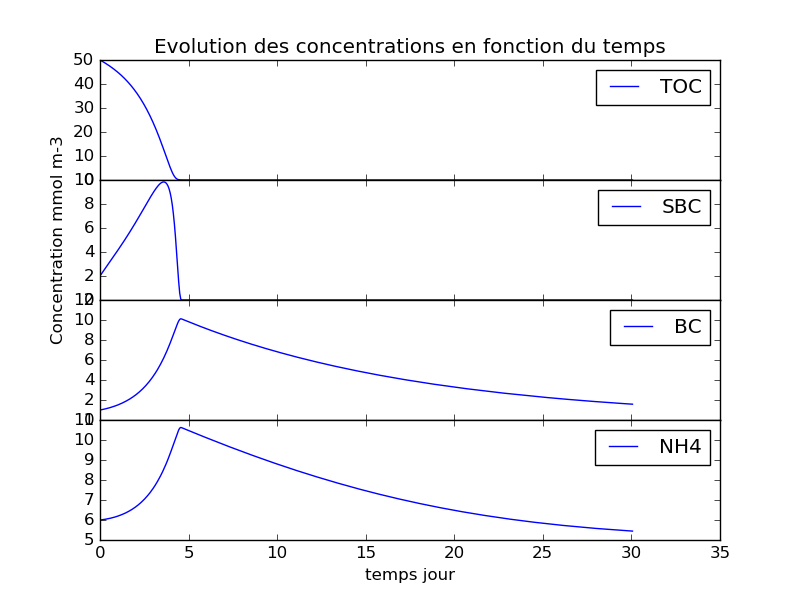
\includegraphics[width=\textwidth]{partie1/Test2.png}
  \caption{Simulation en r\'eduisant la valeur de la constante d'hydrolyse de TOC.
  }
  \label{fig:partie1test2}
\end{figure}

\par{
Dans le deuxième test en a diminué la constante de hydrolyse par rapport à la simulation de référence.
En consequence le terme ec montre des valeurs plus élvées pour les concentrations TOC plus faibles. On obitens
alors l'effet inverse que dans le test 1. La concentration maximale des bactéries et celle d'ammonium plus
tôt. (On peut observer la concentration maximale déjà $t=4.56$.)
}

\FloatBarrier
\newpage
\subsubsection{Test 3}

\begin{figure}[h!]
  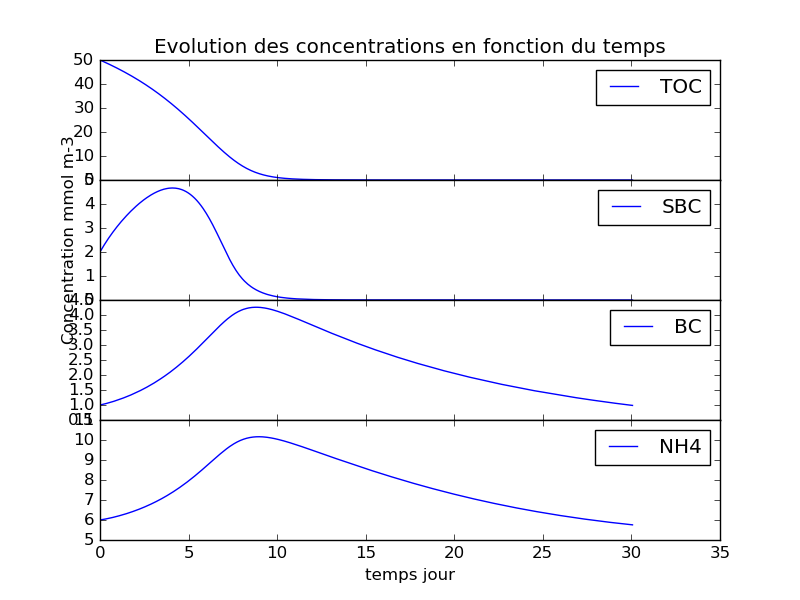
\includegraphics[width=\textwidth]{partie1/Test3.png}
  \caption{Simulation en r\'eduisant la valeur du taux de croissance des bact\'eries
  }
  \label{fig:partie1test3}
\end{figure}

\par{
Dans le troisième test on a diminué le taux de croissance des BC. On restreinds alors la croissance des BC.
Quand il y en a moins des BC, la concentration TOC et SBC métabolisée par bout de temps diminuera. Les
substrats est confinés plus tard. Donc les maximas sont atteinds plus tard.
}

\FloatBarrier
\newpage
\subsubsection{Test 4}

\begin{figure}[h!]
  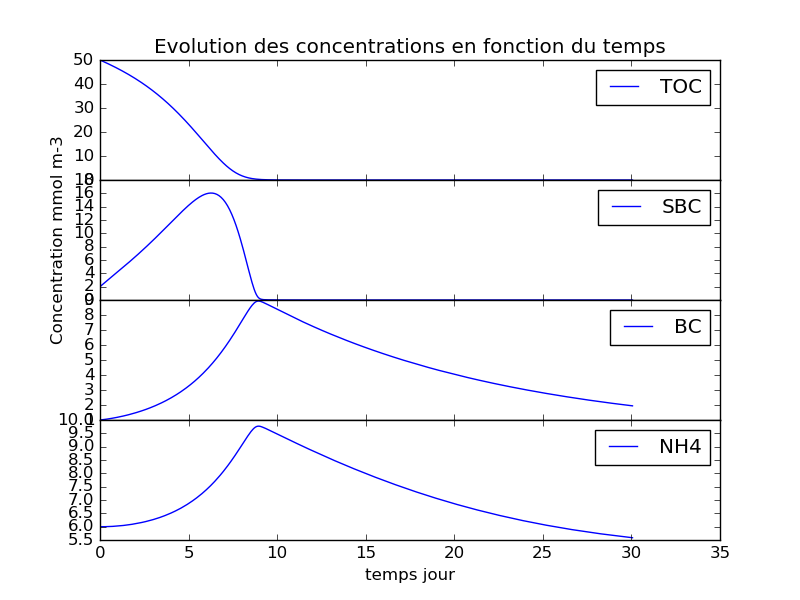
\includegraphics[width=\textwidth]{partie1/Test4.png}
  \caption{Simulation en r\'eduisant la valeur de la constante d'uptake de SBC \`a temp\'erature optimale.}
  \label{fig:partie1test4}
\end{figure}

\par{
Dans le quatrième test on a diminué la constante d'uptake des SBC. En consequénce le terme ubc diminuera et
les BC pouvent métaboliser les SBC moins vite. Du coup le taux de croissance des BC est reduit. On observe
ainsi la même situation que dans le test 3.
}

\FloatBarrier
\newpage
\subsubsection{Test 5}

\begin{figure}[h!]
  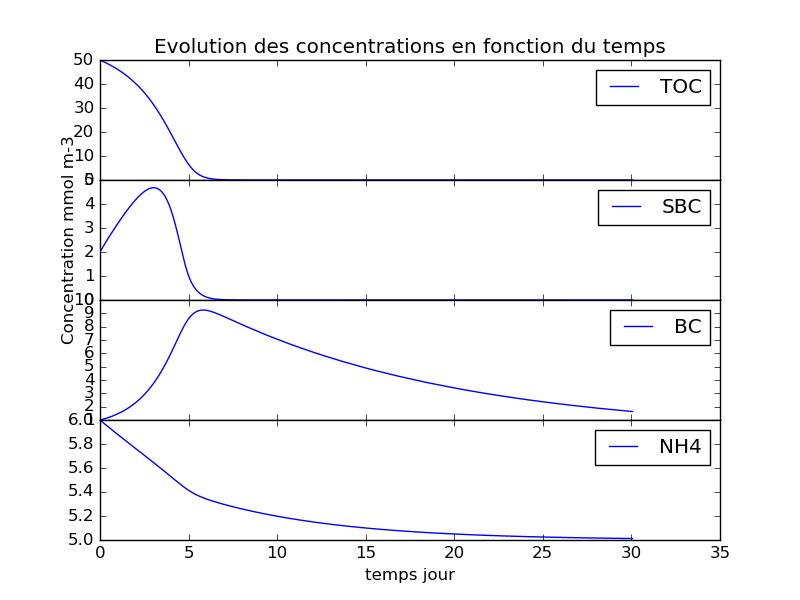
\includegraphics[width=\textwidth]{partie1/Test5.png}
  \caption{Simulation en r\'eduisant la valeur du rapport NC du TOC.}
  \label{fig:partie1test5}
\end{figure}

\par{
Dans cette simulation, seul le rapport N:C de TOC est modifi\'e, et est bien inf\'erieur \`a celui de la
r\'ef\'erence. Ainsi, le terme vNH4 devient n\'egatif, ce qui veut dire que les bact\'eries puisent du NH4
dans leur environnement, et donc que la concentration en NH4 diminue. Il y a deux types de d\'ecroissance de
la concentration en NH4 dans cette simulation. Au d\'ebut et jusque 6 jours, la d\'ecroissance de la
concentration en NH4 est due \`a l'utilisation du NH4 par les bact\'eries, et \`a la nitrification. Apr\`es
6 jours, la concentration en SBC devient nulle, et donc la diminution de la concentration de NH4 n'est plus
due qu'\`a la nitrification. C'est pourquoi, la d\'ecroissance est moins rapide qu'au d\'ebut de la simulation.
On peut noter que la concentration en NH4 va plafonner autour d'une valeur de 5 mmolC.m-3. En effet, la
nitrification est d\'ecrite par une fonction de type Michaelis-Menten avec seuil. Ce seuil correspond \`a la
constante de demi-saturation, qui a une valeur de 5 mmolC.m-3. Comme le rapport N:C de TOC n'a pas d'influence
sur les autres processus, seul l'\'evolution de la concentration en NH4 est modifi\'ee dans cette simulation.
}

\FloatBarrier
\subsubsection{Test 6}

\begin{figure}[h!]
  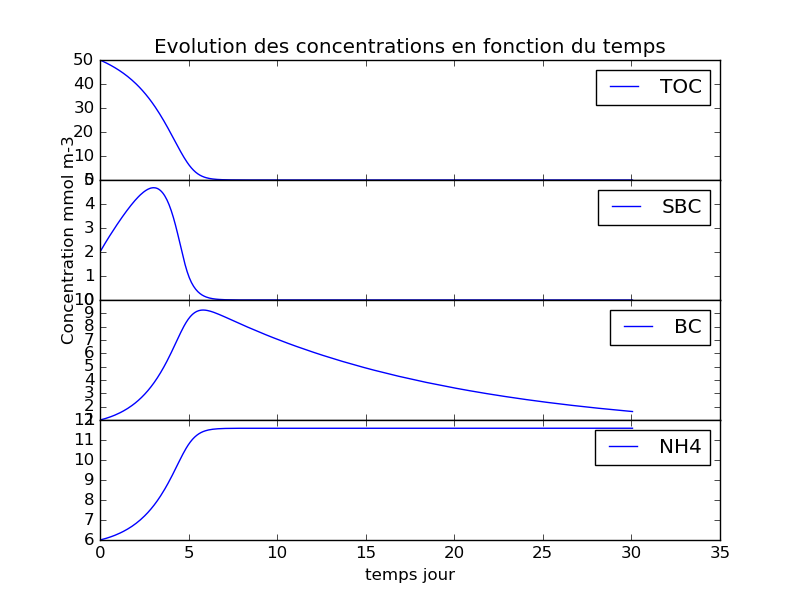
\includegraphics[width=\textwidth]{partie1/Test6.png}
  \caption{Simulation en supprimant l'effet de la nitrification
  }
  \label{fig:partie1test6}
\end{figure}

\par{
Dans cette simulation, le terme de nitrification est nul. Ainsi, seul le terme vNH4 influence l'\'evolution de
la concentration en NH4. Or, ce terme est ici positif, ce qui signifie que les bact\'eries rel\^achent du NH4
dans leur environnement. Ainsi, au d\'ebut de la simulation, la concentration en NH4 augmente jusqu'\`a
atteindre un plafond. Celui-ci est atteint lorsque la concentration en SBC devient nulle. En effet, si la
concentration en SBC devient nulle, alors le terme vNH4 le devient aussi, et donc la concentration en NH4
n'\'evolue plus. Ici aussi, le terme de nitrification n'influence que l'\'evolution de la concentration en
NH4, et donc seul ce processus est diff\'erent, par rapport \`a la r\'ef\'erence.
}

\FloatBarrier
\newpage
\subsection{Conclusion}
\par{
En raison du fait que nous partons d'une quantité limitée de $TOC$ non-régénérable, la population bactérienne
ne peut pas croître indéfiniment. (Ainsi, d'un moment donné, les bactéries souffrent de la faim.)
Pour les simulations infiniment longues, on obtient donc toujours que le TOC est épuisé et la
concentration des bactéries est tombée à $0$. Cela vaut également pour la concentration de SBC.
Seule la concentration de NH4 peut se stabiliser à une concentration plus grandes que $0$.
}
\par{
Puisque le résultat final de la simulation est fixe, les différences qui conduisent à cette situation
sont les plus intéressantes. Ici on peut remarquer quelques différences qui sont principallement dues à
la pénurie du $TOC$. \todo
}
